%%%%%%%%%%%%%%%%%%%% stacks-project-zh.tex %%%%%%%%%%%%%%%%%%%%%%%
% Chinese translation entry point based directly on the complete SVMono
% template in this directory. Build it through the repository Makefile.
%%%%%%%%%%%%%%%%%%%%%%%%%%%%%%%%%%%%%%%%%%%%%%%%%%%%%%%%%%%%%%%%%%

\documentclass[graybox,envcountchap,sectrefs,chinese,oribibl]{svmono}

% Keep the imported template's cover and monograph layout as the visual base.
\usepackage{styles/cover}
\usepackage{styles/stacks-project-zh}
\usepackage{styles/reference-template-compat}
\usepackage{setspace}
\onehalfspacing

\usepackage{type1cm}
\usepackage{graphicx}
\usepackage{multicol}
\usepackage[bottom]{footmisc}
\usepackage{newtxtext}
\usepackage[varvw]{newtxmath}
\usepackage{enumitem}

\makeatletter
\renewcommand*\l@section{\@dottedtocline{1}{1em}{2.6em}}
\makeatother

% Stable project metadata. Build-specific source information is injected by
% the Makefile and model-specific information is supplied by metadata.tex.
\providecommand{\StacksProjectName}{The Stacks Project}
\providecommand{\StacksChineseTitle}{Stacks Project 中文翻译}
\providecommand{\StacksOriginalAuthor}{The Stacks Project Authors}
\providecommand{\StacksProjectURL}{https://stacks.math.columbia.edu/}
\providecommand{\StacksProjectEmail}{stacks.project@gmail.com}
\providecommand{\StacksOriginalCopyright}{Copyright \textcopyright\ 2005--2025 Johan de Jong}
\providecommand{\StacksLicenseName}{GNU Free Documentation License 1.2 或更高版本}

\providecommand{\StacksSourceRevision}{unknown}
\providecommand{\StacksSourceDate}{unknown}
\providecommand{\TranslationModelName}{\TranslationModel}
\providecommand{\TranslationMaintainer}{OpenSSL}
\providecommand{\TranslationStatus}{工作草稿}
\providecommand{\TranslationNotice}{本译本为非官方中文翻译；如有歧义，以英文原作为准。}


\providecommand{\TranslationModel}{template}
\edef\TranslationModelDirectory{translations/\TranslationModel}

\IfFileExists{\TranslationModelDirectory/metadata.tex}{%
  % Smoke-test metadata. Copy this directory when starting a real model output.
\renewcommand{\TranslationModelName}{模板冒烟测试}
\renewcommand{\TranslationMaintainer}{OpenSSL}
\renewcommand{\TranslationStatus}{仅用于 LaTeX 模板验证，不是正式译文}
\renewcommand{\TranslationNotice}{本目录只验证版式和源文件兼容性；任何示例文字均不得视为 Stacks Project 的中文译文。}

}{%
  \PackageError{stacks-project-zh}
    {Missing \TranslationModelDirectory/metadata.tex}
    {Create metadata.tex for the selected translation model.}
}

% Resolve model-specific figures before shared template images.
\graphicspath{{\TranslationModelDirectory/images/}{images/}}

\hypersetup{
  pdftitle={\StacksChineseTitle},
  pdfauthor={\StacksOriginalAuthor},
  pdfsubject={基于英文源提交 \StacksSourceRevision{} 的中文翻译（\TranslationModelName）},
  pdfkeywords={Stacks Project, 中文翻译, 代数几何}
}

\makeindex

\begin{document}

% The following sequence is inherited from the complete Springer template:
% custom cover, SVMono title page, front matter, main matter, and back matter.
\title{\StacksChineseTitle}
\subtitle{\StacksProjectName}
\edition{英文源 \StacksSourceRevision\quad \StacksSourceDate}
\bookseries{The Stacks Project\quad 中文翻译}
\author{\StacksOriginalAuthor}
\coverfooter{翻译模型：\TranslationModelName}
\makecover
\maketitle

\frontmatter
% The reference template supports dedication, foreword, acknowledgement and
% acronym pages. A translation model may provide all of them in frontmatter.tex.
\IfFileExists{\TranslationModelDirectory/frontmatter.tex}{%
  % Optional model-specific front matter. Examples:
% % Optional SVMono dedication page. Load this from a model frontmatter.tex
% only after replacing the sample sentence with approved project text.
\begin{dedication}
此处填写该翻译版本的题献文字。
\end{dedication}

% % Optional SVMono foreword page. The old project's four edition-specific
% forewords are intentionally not part of the Stacks Project template.
\foreword[译者前言]

此处填写该翻译模型经过审核的译者前言。

\vspace{\baselineskip}
\begin{flushright}
\TranslationMaintainer
\end{flushright}

% % Optional standalone acknowledgement chapter.
\extrachap{致谢}

此处列出该翻译版本的校订者、工具和其他贡献者。

% % Optional list of acronyms/symbols using SVMono's enhanced description list.
\extrachap{缩略语与符号}

\begin{description}[style=multiline,labelwidth=4em,leftmargin=5em]
  \item[QCoh] 拟凝聚层范畴。
  \item[Spec] 环的谱。
\end{description}


}{}
\extrachap{来源、版权与翻译说明}
\addcontentsline{toc}{chapter}{来源、版权与翻译说明}

\noindent
本书是 \StacksProjectName{} 的中文翻译排版。英文原作是一个协作式开放数学
项目，项目主页为 \url{\StacksProjectURL}，联系邮箱为
\href{mailto:\StacksProjectEmail}{\nolinkurl{\StacksProjectEmail}}。

\begin{description}
  \item[英文原作] \StacksOriginalAuthor
  \item[原作版权] \StacksOriginalCopyright
  \item[英文源版本] 提交 \texttt{\StacksSourceRevision}（\StacksSourceDate）
  \item[翻译目录] \nolinkurl{springer-template/translations/\TranslationModel}
  \item[翻译模型] \TranslationModelName
  \item[译本维护] \TranslationMaintainer
  \item[翻译状态] \TranslationStatus
\end{description}

\noindent
英文原作依照 \StacksLicenseName{} 发布，无不变章节、无封面文字、无封底文字；
中文翻译属于该许可证所称的修改版本，并应在相同许可证条件下分发。正式发布的
完整译本必须随附 GNU Free Documentation License 全文。

\medskip\noindent
\TranslationNotice

\medskip\noindent
本书以本目录内的 Springer SVMono 完整模板为排版基础，但不是 Springer 出版物，
也不代表 Springer 或英文 Stacks Project 对本中文翻译的认可。

\preface

Stacks Project 旨在从交换代数与代数几何的基础出发，逐步建立概形、代数空间
以及代数栈理论所需的系统性参考资料。英文原作以在线阅读为主要使用方式，并以
稳定标签和大量内部链接连接分布在各章中的定义、引理与定理。

本中文版本保留原作的数学公式、环境、引用键和永久标签，只翻译可见的叙述性
文字。不同翻译模型的结果分别保存在独立目录中，共享同一套 Springer 中文排版
模板，以便逐章比较、校订和重新构建。

当前 PDF 使用的模型为“\TranslationModelName”，状态为“\TranslationStatus”。
翻译中的任何错误不属于英文原作者；遇到歧义时应核对英文原作及对应的永久标签。

\vspace{\baselineskip}
\begin{flushright}
Stacks Project 中文翻译仓库维护者
\end{flushright}

\tableofcontents

\mainmatter
\IfFileExists{\TranslationModelDirectory/contents.tex}{%
  % Book-native chapter manifest for this translation model.
\chapter{模板兼容性检查}
\label{template-chapter-check}

\section{中文、公式和 Stacks 数学宏}
\label{template-section-macros}

中文正文、行内公式 $X \longrightarrow Y$ 和常用算子应能混合排版。例如
$\Spec(R)$、$\Hom_R(M,N)$、$\SheafExt^1(\mathcal F,\mathcal G)$、
$\QCohstack$、$\etale$ 与 $\colim_i M_i$ 均来自英文 harvest 的共享前导宏。

\begin{definition}[排版测试]
\label{template-definition-typesetting}
这是一个用于推进共享 \texttt{subsection} 计数器的定义环境。
\end{definition}

\begin{equation}
\label{template-equation-polynomial}
  f(x)=x^2+1.
\end{equation}

公式~\ref{template-equation-polynomial}、定义~\ref{template-definition-typesetting}
以及本章第~\ref{template-section-diagrams}~节的交叉引用都应正确。

标准 \texttt{matrix} 环境和粗体矩阵命令不能冲突：
\[
  \begin{matrix}
    a & b \\
    c & d
  \end{matrix}
  \qquad \mat{A}.
\]

参照入口中的数学宏包和辅助命令也应可直接使用：
\[
  \diag{1,2},\qquad
  \closure{U},\qquad
  \seg{0}{1},\ \segl{0}{1},\ \segr{0}{1},\ \seglr{0}{1},\qquad
  \dv{f}{x}.
\]
量纲命令 \SI{3}{\metre}、小写罗马数字 \romannum{4}，以及
\texttt{NiceMatrix} 环境均应正常：
\[
  \begin{NiceMatrix}
    1 & 0 \\
    0 & 1
  \end{NiceMatrix}.
\]

\section{定理、证明和编辑元数据}
\label{template-section-theorems}

\begin{theorem}[示例定理]
\label{template-theorem-example}
定理标题、编号和中文正文应当正常显示。
\end{theorem}

\begin{proof}
证明环境应使用中文标题，并在结尾显示证毕符号。
\end{proof}

\begin{lemma}
\label{template-lemma-example}
引理与定理共用 Stacks Project 的 \texttt{subsection} 计数器。
\end{lemma}

\begin{proposition}
命题环境可用。
\end{proposition}

\begin{exercise}
\label{template-solution}
练习环境可用，并为可选的解答章节提供稳定标签。
\end{exercise}

\begin{situation}
\label{template-situation-example}
英文源文件特有的 \texttt{situation} 环境可用。
\end{situation}

\begin{remark}
单个注记环境可用。
\end{remark}

\begin{remarks}
复数形式的注记环境也可用。
\end{remarks}

\begin{reference}
这段编辑性参考信息不应出现在成书 PDF 中。
\end{reference}
\begin{slogan}
这段口号元数据不应出现在成书 PDF 中。
\end{slogan}
\begin{history}
这段历史元数据不应出现在成书 PDF 中。
\end{history}

\section{交换图、标签链接和索引}
\label{template-section-diagrams}

Xy-pic 交换图应能直接沿用英文源文件的写法：
\[
\xymatrix{
  X \ar[r]^f \ar[d]_g & Y \ar[d]^h \\
  Z \ar[r]_k & W
}
\]

永久标签链接示例：\StacksTag{0000}。项目引用示例见~\cite{stacks-project}。

\index{Stacks Project}
\index{中文排版}
索引应能生成，且不产生按 UTF-8 字节计算的乱码分组标题。


}{%
  \PackageError{stacks-project-zh}
    {Missing \TranslationModelDirectory/contents.tex}
    {List the selected model's translated chapters in contents.tex.}
}
% Keep the reference appendix hook, scoped per translation model.
\IfFileExists{\TranslationModelDirectory/appendices.tex}{%
  % Optional model-specific appendices. Example:
% % Optional appendix skeleton preserving the reference template's chapter,
% equation, figure and table layout surface.
\appendix
\chapter{附录标题}
\label{appendix-template}

\section{补充材料}
\label{appendix-template-section}

此处填写该翻译版本的补充材料。公式、图和表仍使用 SVMono 的原生环境。

\begin{equation}
  \label{appendix-template-equation}
  X \longrightarrow Y.
\end{equation}

\begin{figure}[t]
  \sidecaption[t]
  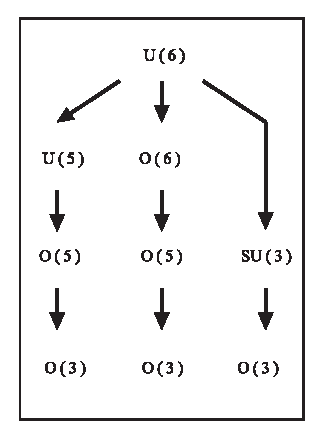
\includegraphics[scale=.65]{images/figure}
  \caption{参照模板附带的占位图。}
  \label{appendix-template-figure}
\end{figure}

\begin{table}
  \caption{表格版式占位示例。}
  \label{appendix-template-table}
  \begin{tabular}{p{3cm}p{7cm}}
    \hline\noalign{\smallskip}
    项目 & 说明 \\
    \noalign{\smallskip}\hline\noalign{\smallskip}
    英文源 & 相邻的 harvest 仓库 \\
    中文译文 & 当前翻译模型目录 \\
    \noalign{\smallskip}\hline
  \end{tabular}
\end{table}


}{}

\backmatter
% Use the bibliography maintained by the adjacent English harvest instead of
% copying a stale project-specific bibliography into this template.
\bibliographystyle{styles/spmpsci}
\nocite{stacks-project}
\bibliography{my}

\IfFileExists{\TranslationModelDirectory/backmatter.tex}{%
  % Optional model-specific back matter. Examples:
% % Optional glossary using the SVMono run-in heading style.
\extrachap{术语表}

\runinhead{术语} 此处填写术语的中文释义及采用该译名的说明。

\runinhead{永久标签} Stacks Project 用于稳定链接定义、引理和定理的标识符。

% % Optional solutions chapter. Replace labels with labels from translated
% exercises before including it from a model backmatter.tex.
\extrachap{解答}

\begin{sol}{template-solution}
此处填写练习解答。
\end{sol}


}{}
\printindex

\end{document}
